\documentclass[11pt, a4paper, twoside]{article}   	% use "amsart" instead of "article" for AMSLaTeX format

\usepackage{geometry}                		% See geometry.pdf to learn the layout options. There are lots.
\usepackage{pdfpages}
\usepackage{caption}
\usepackage{minted}
\usepackage[german]{babel}			% this end the next are needed for german umlaute
\usepackage[utf8]{inputenc}
\usepackage{color}
\usepackage{graphicx}
\usepackage{titlesec}
\usepackage{fancyhdr}
\usepackage{lastpage}
\usepackage{hyperref}
\usepackage[autostyle=false, style=english]{csquotes}
\usepackage{mathtools}
\usepackage{tabularx}
% http://www.artofproblemsolving.com/wiki/index.php/LaTeX:Symbols#Operators
% =============================================
% Layout & Colors
% =============================================
\geometry{
   a4paper,
   total={210mm,297mm},
   left=20mm,
   right=20mm,
   top=20mm,
   bottom=30mm
 }	

\definecolor{myred}{rgb}{0.8,0,0}
\definecolor{mygreen}{rgb}{0,0.6,0}
\definecolor{mygray}{rgb}{0.5,0.5,0.5}
\definecolor{mymauve}{rgb}{0.58,0,0.82}

\setcounter{secnumdepth}{4}


% the default java directory structure and the main packages
\newcommand{\srcDirGenerator}{../src/T4/ClassGenerator}
\newcommand{\srcDirClone}{../src/T4/CloningGenerator}
\newcommand{\srcDirJavaSrc}{../src/gp2-svg-generator/src/main/java}
\newcommand{\srcDirJavaRes}{../src/gp2-svg-generator/src/main/resources}
\newcommand{\srcDirJavaOut}{../src/gp2-svg-generator/output}
\newcommand{\imageDir}{images}
% =============================================
% Code Settings
% =============================================
\newenvironment{code}{\captionsetup{type=listing}}{}
\newmintedfile[cppSourceFile]{cpp}{
	linenos=true, 
	frame=single, 
	breaklines=true, 
	tabsize=2,
	numbersep=5pt,
	xleftmargin=10pt,
	baselinestretch=1,
	fontsize=\footnotesize
}
\newmintedfile[xmlFile]{xml}{
	linenos=true, 
	frame=single, 
	breaklines=true, 
	tabsize=2,
	numbersep=5pt,
	xleftmargin=10pt,
	baselinestretch=1,
	fontsize=\footnotesize
}
\newmintedfile[javaFile]{java}{
	linenos=true, 
	frame=single, 
	breaklines=true, 
	tabsize=2,
	numbersep=5pt,
	xleftmargin=10pt,
	baselinestretch=1,
	fontsize=\footnotesize
}
\newmintedfile[jsonFile]{json}{
	linenos=true, 
	frame=single, 
	breaklines=true, 
	tabsize=2,
	numbersep=5pt,
	xleftmargin=10pt,
	baselinestretch=1,
	fontsize=\footnotesize
}
\newmintinline[inlineCpp]{cpp}{}
\newminted[cppSource]{cpp}{
	breaklines=true, 
	tabsize=2,
	autogobble=true,
	breakautoindent=false
}

\newcommand{\xvdash}[1]{%
  \vdash^{\mkern-10mu\scriptscriptstyle\rule[-.9ex]{0pt}{0pt}#1}%
}

% =============================================
% Page Style, Footers & Headers, Title
% =============================================
\title{Übung 3}
\author{Thomas Herzog}

\lhead{Übung 3}
\chead{}
\rhead{
\includegraphics[scale=0.10]{FHO_Logo_Students.jpg}}

\lfoot{S1610454013}
\cfoot{}
\rfoot{ \thepage / \pageref{LastPage} }
\renewcommand{\footrulewidth}{0.4pt}
% =============================================
% D O C U M E N T     C O N T E N T
% =============================================
% =============================================
% 2016.10.13: 1 
% 2016.10.14: 2
% =============================================
\pagestyle{fancy}
\begin{document}
\setlength{\headheight}{15mm}
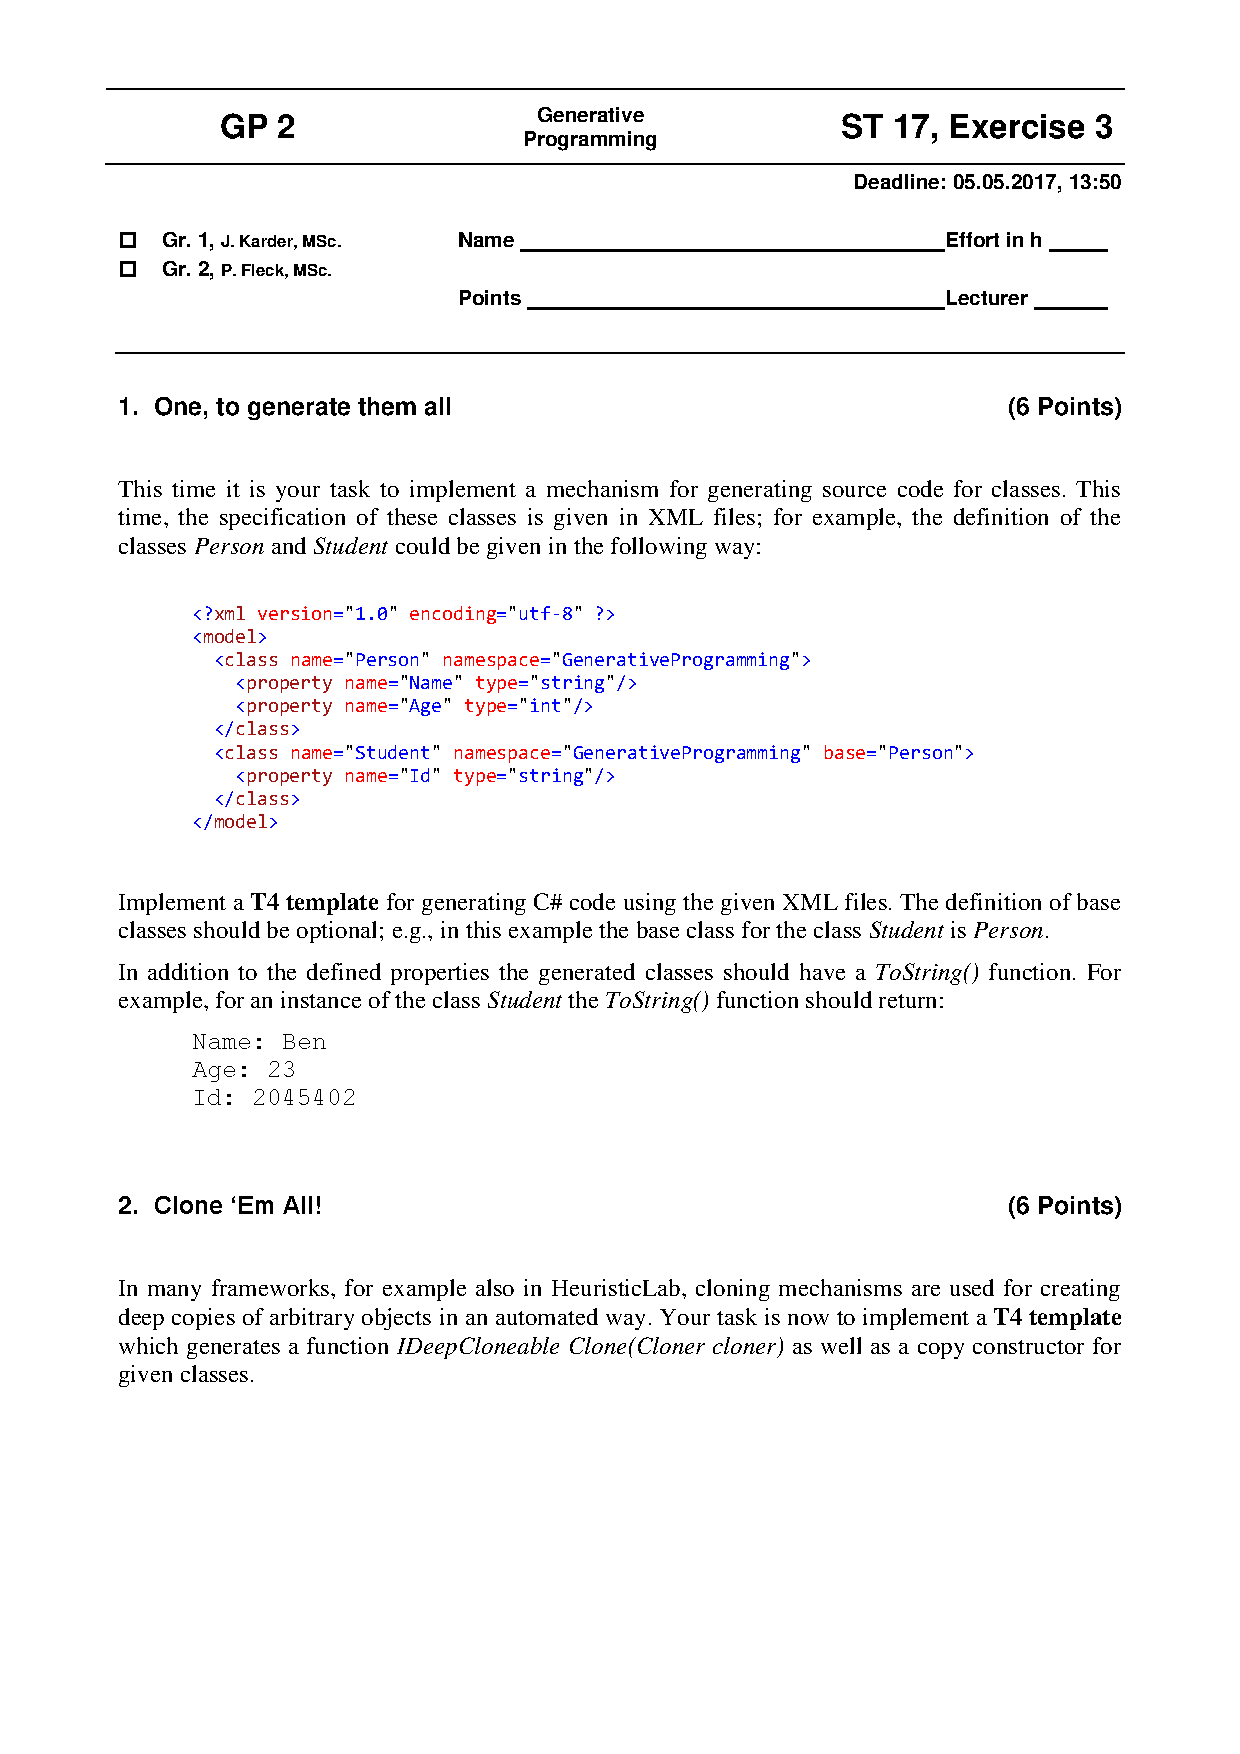
\includepdf[pages={1,2,3,4,5}]{GP_A03.pdf}

\section{One, to generate them all}
Dieser Abschnitt beschäftigt sich mit der Dokumentation der Aufgabenstellung \emph{One, to generate them all}.
\subsection{Lösungsidee} 
Um von den \emph{XML-Tag}-Namen und dessen Attributnamen unabhängig zu sein, sollen die \emph{XML-Tag}-Namen und dessen Attributnamen in Konstanten ausgelagert werden und sollen bei der Navigation durch das \emph{XML}-Dokument verwendet werden, um die \emph{XML-Tags} sowie dessen Attributnamen zu adressieren. Die Unabhängigkeit von der Struktur des \emph{XML}-Dokuments wird aber nicht möglich sein.
\newline
\newline
Da die im \emph{XML}-Dokument definierten Klassen sich im selben Namensraum befinden können, sollen die definierten Klassen nach den Namensräumen gruppiert werden, damit die Namensräume nicht mehrfach in den generierten Klassen definiert werden müssen. Um das zu realisieren soll \emph{Linq} verwendet werden. Um sich zu viele \emph{If}-Anweisungen im \emph{T4-Template} zu vermeiden soll mit dem \emph{?} Operator gearbeitet werden, um die resultierenden Zeichenketten des C\# Quelltextes zu generieren. Dadurch soll das \emph{T4-Template} übersichtlicher werden, da meiner Meinung nach das Verwenden von zu vielen \emph{If}-Anweisungen das \emph{Template} unübersichtlich macht.
\newline
\newline
Zusätzlich zu den verlangten Attributen der \emph{XML-Tags} wurde noch auf Klassenebene ein \emph{Modifier}-Attribut eingeführt, womit auch abstrakte Klassen definiert werden können.  
\newline
\newline
Die Methode \emph{ToString} wurde so implementiert, dass wenn es eine Basisklasse gibt, zuerst an diese Basisklasse delegiert wird und dann erst die Ausgabe der konkreten Klasse erfolgt, wobei am Anfang einer jeder \emph{ToString} Methodenimplementierung immer die der Klassennamen ausgegeben wird.     

\subsection{Quelltexte}
Folgender Abschnitt enthält das \emph{T4-Template} und das Testprogramm.
\begin{code}
	\caption{ClassGenerator.tt}
	\cppSourceFile{\srcDirGenerator/ClassGenerator.tt}
	\label{src:class-generator-tt}
\end{code}

\begin{code}
	\caption{Model.xml}
	\xmlFile{\srcDirGenerator/Model.xml}
	\label{src:model-xml}
\end{code}

\begin{code}
	\caption{Program.cs}
	\cppSourceFile{\srcDirGenerator/Program.cs}
	\label{src:program-cs}
\end{code}

\subsection{Tests}
Folgender Abschnitt enthält die Tests der Aufgabenstellung in Form der generierten Quelltexte sowie der Ausgaben des Testprogramms.

\begin{code}
	\caption{ClassGenerator.cs}
	\cppSourceFile{\srcDirGenerator/ClassGenerator.cs}
	\label{src:class-generator-cs}
\end{code}

\begin{figure}[h]
	\centering
	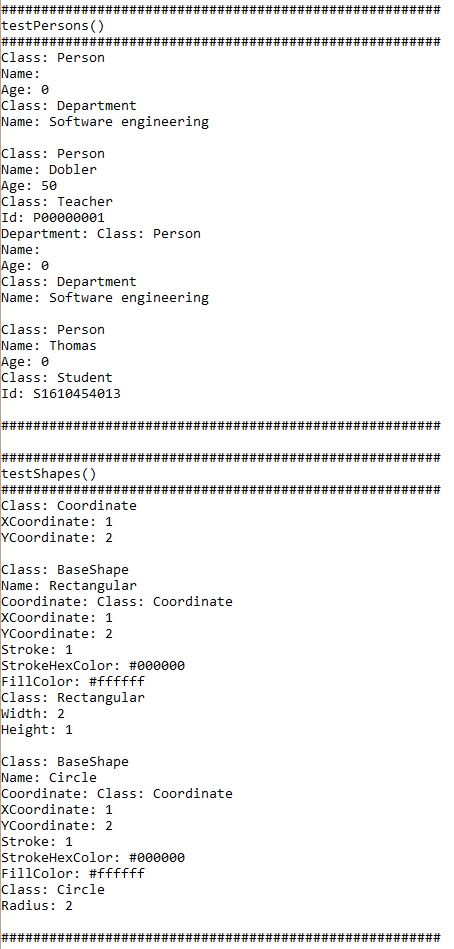
\includegraphics[scale=0.73]{\imageDir/class-generator.JPG}
	\caption{\emph{Class} Generator Testausgabe}
	\label{fig:class-generator}
\end{figure}
\ \newpage

\section{Clone 'Em All}
Dieser Abschnitt beschäftigt sich mit der Dokumentation der Aufgabenstellung \emph{Clone 'Em All}.
\subsection{Lösungsidee} Diese Aufgabenstellung wurde bereits in der Übung implementiert und nachträglich formatiert und einige Kommentare eingefügt.

\subsection{Quelltexte}
In diesem Abschnit werden nur die selbst implementierten Quelltexte und das \emph{T4-Template} angeführt.

\begin{code}
	\caption{CloningGenerator.tt}
	\cppSourceFile{\srcDirClone/CloningGenerator.tt}
	\label{src:cloning-generator-tt}
\end{code}

\begin{code}
	\caption{A.cs}
	\cppSourceFile{\srcDirClone/A.cs}
	\label{src:a-cs}
\end{code}

\begin{code}
	\caption{B.cs}
	\cppSourceFile{\srcDirClone/B.cs}
	\label{src:b-cs}
\end{code}

\begin{code}
	\caption{Program.cs}
	\cppSourceFile{\srcDirClone/Program.cs}
	\label{src:cloning-program-cs}
\end{code}

\subsection{Tests} 
Dieser Abschnitt enthält die Tests in Form von den generierten Quelltexten und der Ausgabe des Testprogramms.

\begin{code}
	\caption{CloningGenerator.cs}
	\cppSourceFile{\srcDirClone/CloningGenerator.cs}
	\label{src:cloning-generator-cs}
\end{code}

\begin{figure}[h]
	\centering
	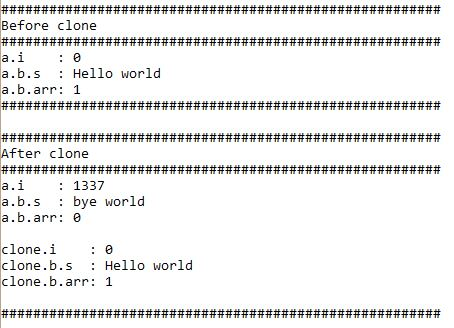
\includegraphics[scale=0.73]{\imageDir/clone-generator.JPG}
	\caption{\emph{Clone} Generator Testausgabe}
	\label{fig:clone-generator}
\end{figure}

\section{SVG Generator}
Dieser Abschnitt beschäftigt sich mit der Dokumentation der Aufgabenstellung \emph{SVG Generator}.
\subsection{Lösungsidee} Es sollen zwei \emph{Exception}-Klassen implementiert werden, wobei eine \emph{Exception}-Klasse einen durch den Generator verursachten Fehler repräsentiert und die andere \emph{Exception}-Klasse einen durch eine \emph{Shape} verursachten Fehler repräsentiert.
\newline
\newline
Es soll jeweils eine Schnittstelle für die Repräsentation eines \emph{Generators} und eines \emph{Shapes} implementiert werden um beide Aspekte von ihren Implementierungen zu trennen. Es sollen abstrakte Klassen für die Generatoren und die \emph{Shapes} implementiert werden, welche die gemeinsame Funktionalität kapseln. Die implementierten Generatoren und \emph{Shapes} sollen von diesen Klassen erben und die spezifischen Funktionalitäten und Zustände implementieren.
\newline
\newline
Damit nicht zu viele Klassendateien für die SVG Generatoren angelegt werden sollen die Generatorenklassen als statische innere Klassen in einer Klasse gekapselt werden. Es sollen die folgenden SVG-\emph{Tags}
\begin{itemize}
	\item\emph{PointShape},
	\item\emph{LineShape},
	\item\emph{RectangularShape} und
	\item\emph{TextShape}
\end{itemize}   
implementiert werden.
\newpage
Da die \emph{Shapes} unabhängig von ihrer konkreten Repräsentation sind, sollen die \emph{Shape}-Klassen im \emph{api Package} organisiert werden, damit sie auch für andere \emph{Temlate-Engines} nutzbar sind.
\newline
\newline
Um sich die \emph{Getter} und \emph{Setter}-Methoden zu ersparen wurde die Bibliothek \emph{lombok} verwendet, die über Annotationen die \emph{Getter} und \emph{Setter}-Methoden generiert, wobei der \emph{Compiler} instrumentiert wird. Siehe folgenden Link wie \emph{lombok} verwendet wird und wie die Bibliothek \emph{lombok} in eine \emph{IDE} integriert wird \url{https://projectlombok.org/download.html}.
\newline
\newline
Ohne diese Integration von der Bibliothek \emph{lombok} kann das Program nicht in einer IDE gebaut werden.
\newline
\newline
Die Abbildung \ref{fig:svg-project-structure} zeigt die Implementierte Projektstruktur und Organisation der \emph{Packages}.
\newline
\begin{figure}[h]
	\centering
	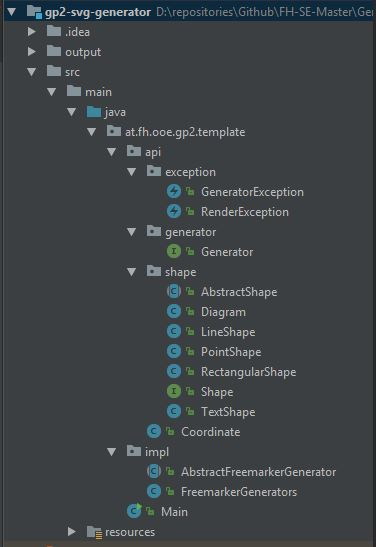
\includegraphics[scale=1]{\imageDir/svg-project-structure.JPG}
	\caption{Projektstruktur}
	\label{fig:svg-project-structure}
\end{figure}
\ \newpage

\subsection{Quelltexte}
\begin{code}
	\caption{GeneratorException.java}
	\javaFile{\srcDirJavaSrc/at/fh/ooe/gp2/template/api/exception/GeneratorException.java}
	\label{src:generatorexception-java}
\end{code}

\begin{code}
	\caption{GeneratorException.java}
	\javaFile{\srcDirJavaSrc/at/fh/ooe/gp2/template/api/exception/RenderException.java}
	\label{src:renderexception-java}
\end{code}

\begin{code}
	\caption{Generator.java}
	\javaFile{\srcDirJavaSrc/at/fh/ooe/gp2/template/api/generator/Generator.java}
	\label{src:generator-java}
\end{code}

\begin{code}
	\caption{Shape.java}
	\javaFile{\srcDirJavaSrc/at/fh/ooe/gp2/template/api/shape/Shape.java}
	\label{src:shape-java}
\end{code}

\begin{code}
	\caption{Coordinate.java}
	\javaFile{\srcDirJavaSrc/at/fh/ooe/gp2/template/api/Coordinate.java}
	\label{src:coordinate-java}
\end{code}

\begin{code}
	\caption{AbstractShape.java}
	\javaFile{\srcDirJavaSrc/at/fh/ooe/gp2/template/api/shape/AbstractShape.java}
	\label{src:shape-java}
\end{code}

\begin{code}
	\caption{Diagram.java}
	\javaFile{\srcDirJavaSrc/at/fh/ooe/gp2/template/api/shape/Diagram.java}
	\label{src:diagram-shape-java}
\end{code}

\begin{code}
	\caption{PointShape.java}
	\javaFile{\srcDirJavaSrc/at/fh/ooe/gp2/template/api/shape/PointShape.java}
	\label{src:point-shape-java}
\end{code}

\begin{code}
	\caption{LineShape.java}
	\javaFile{\srcDirJavaSrc/at/fh/ooe/gp2/template/api/shape/LineShape.java}
	\label{src:line-shape-java}
\end{code}

\begin{code}
	\caption{RectangularShape.java}
	\javaFile{\srcDirJavaSrc/at/fh/ooe/gp2/template/api/shape/RectangularShape.java}
	\label{src:rectangular-shape-java}
\end{code}

\begin{code}
	\caption{TextShape.java}
	\javaFile{\srcDirJavaSrc/at/fh/ooe/gp2/template/api/shape/TextShape.java}
	\label{src:text-shape-java}
\end{code}

\begin{code}
	\caption{AbstractFreemarkerGenerator.java}
	\javaFile{\srcDirJavaSrc/at/fh/ooe/gp2/template/impl/generator/AbstractFreemarkerGenerator.java}
	\label{src:abstract-freemarker-generator-java}
\end{code}

\begin{code}
	\caption{FreemarkerGenerators.java}
	\javaFile{\srcDirJavaSrc/at/fh/ooe/gp2/template/impl/generator/FreemarkerGenerators.java}
	\label{src:freemarker-generators-java}
\end{code}

\begin{code}
	\caption{Main.java}
	\javaFile{\srcDirJavaSrc/at/fh/ooe/gp2/template/Main.java}
	\label{src:main-java}
\end{code}

\begin{code}
	\caption{diagram.ftl}
	\xmlFile{\srcDirJavaRes/templates/shapes/svg/diagram.ftl}
	\label{src:diagram-ftl}
\end{code}

\begin{code}
	\caption{point.ftl}
	\xmlFile{\srcDirJavaRes/templates/shapes/svg/point.ftl}
	\label{src:point-ftl}
\end{code}

\begin{code}
	\caption{line.ftl}
	\xmlFile{\srcDirJavaRes/templates/shapes/svg/line.ftl}
	\label{src:line-ftl}
\end{code}

\begin{code}
	\caption{rect.ftl}
	\xmlFile{\srcDirJavaRes/templates/shapes/svg/rect.ftl}
	\label{src:rect-ftl}
\end{code}

\begin{code}
	\caption{text.ftl}
	\xmlFile{\srcDirJavaRes/templates/shapes/svg/text.ftl}
	\label{src:text-ftl}
\end{code}

\subsection{Tests}
Dieser Abschnitt beinhaltet die generierten SVG-Dateien und die dazugehörigen Bilder.
\begin{code}
	\caption{boxes.svg}
	\xmlFile{\srcDirJavaOut/boxes.svg}
	\label{src:boxes-svg}
\end{code}

\begin{figure}[h]
	\centering
	
\includegraphics[scale=1]{\imageDir/svg-boxes.JPG}
	\caption{\emph{Boxes}}
	\label{fig:svg-boxes}
\end{figure}

\begin{code}
	\caption{points.svg}
	\xmlFile{\srcDirJavaOut/points.svg}
	\label{src:boxes-svg}
\end{code}

\begin{figure}[h]
	\centering
	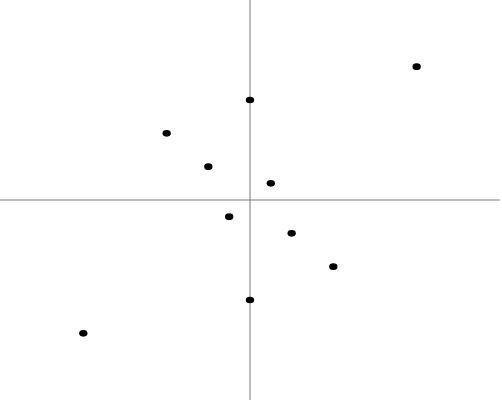
\includegraphics[scale=1]{\imageDir/svg-points.JPG}
	\caption{\emph{Points}}
	\label{fig:svg-points}
\end{figure}

\begin{code}
	\caption{lines.svg}
	\xmlFile{\srcDirJavaOut/lines.svg}
	\label{src:lines-svg}
\end{code}

\begin{figure}[h]
	\centering
	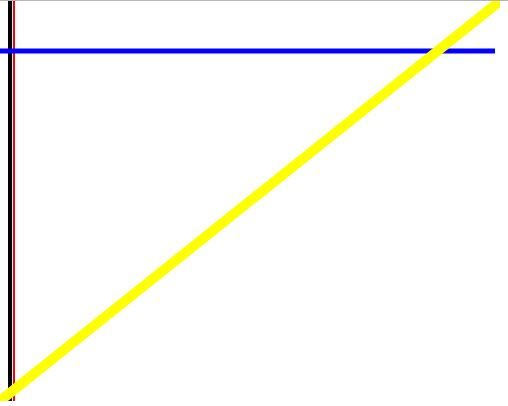
\includegraphics[scale=0.9]{\imageDir/svg-lines.JPG}
	\caption{\emph{Lines}}
	\label{fig:svg-lines}
\end{figure}
\ \newpage

\begin{code}
	\caption{all.svg}
	\xmlFile{\srcDirJavaOut/all.svg}
	\label{src:all-svg}
\end{code}

\begin{figure}[h]
	\centering
	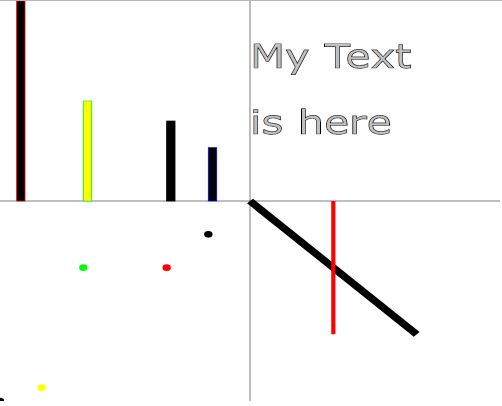
\includegraphics[scale=1]{\imageDir/svg-all.JPG}
	\caption{\emph{All}}
	\label{fig:svg-all}
\end{figure}

\end{document}